\noindent

\includegraphics[height=1.25cm]{images/pictograms/replication}

\includegraphics[height=1.25cm]{images/pictograms/benchmark}

\includegraphics[height=1.25cm]{images/pictograms/under_construction}

\includegraphics[height=1.25cm]{images/pictograms/FEM}

\includegraphics[height=1.25cm]{images/pictograms/paraview}

%%%%%%%%%%%%%%%%%%%%%%%%%%%%%%%%%%%%%%%%%%%%%%%%%%%%%%%%%%%%%%%%%%%%%%%%%%%%%%%%%%%%%%%%%%%%%%%%%%%

\begin{flushright} {\tiny {\color{gray} \tt python\_codes/fieldstone\_161/text.tex}} \end{flushright}

%\lstinputlisting[language=bash,basicstyle=\small]{python_codes/template_keywords.key}

\par\noindent\rule{\textwidth}{0.4pt}

\begin{center}
\inpython
{\small Code: \url{https://github.com/cedrict/fieldstone/tree/master/python_codes/fieldstone_161}}
\end{center}

\par\noindent\rule{\textwidth}{0.4pt}

%%%%%%%%%%%%%%%%%%%%%%%%%%%%%%%%%%%%%%%%%%%%%%%%%%%%%%%%%%%%%%%%%%%%%%%%%%%%%%%%%%%%%%%%%%%%%%%%%%%

We here consider the $Q_{k+1,k}\times Q_{k,k+1} \times Q_{k}^-$ element introduced 
by \textcite{huzh11} (2011) which follows \textcite{zhan09} (2009).
The shape functions in 2D are in derived in Section~\ref{ss:qqq_elt}. 

The list of velocity degrees of freedom per element is as follows:
\[
\vec{\cal V} = (u_1,v_1,u_2,v_2,u_3,v_3,u_4,v_4,u_5,v_5,u_6,v_6)
\]
with the following internal numbering
\begin{verbatim}

u dofs      v dofs

4--6--3     4-----3
|     |     |     |
|     |     5     6
|     |     |     |
1--5--2     1-----2

\end{verbatim}
It is rather interesting to note that the location of the 'extra' 
nodes for u and v are opposite of those for the Fortin $Q_1^+\times P_0$ element, see
Section \ref{MMM-ss:Q1pP02D} (see also \stone~80).

We start with a simple $4\times 3$ element mesh.
Bubble $u$ dofs are represented in red and bubble $v$ dofs are shown in blue.


\begin{center}
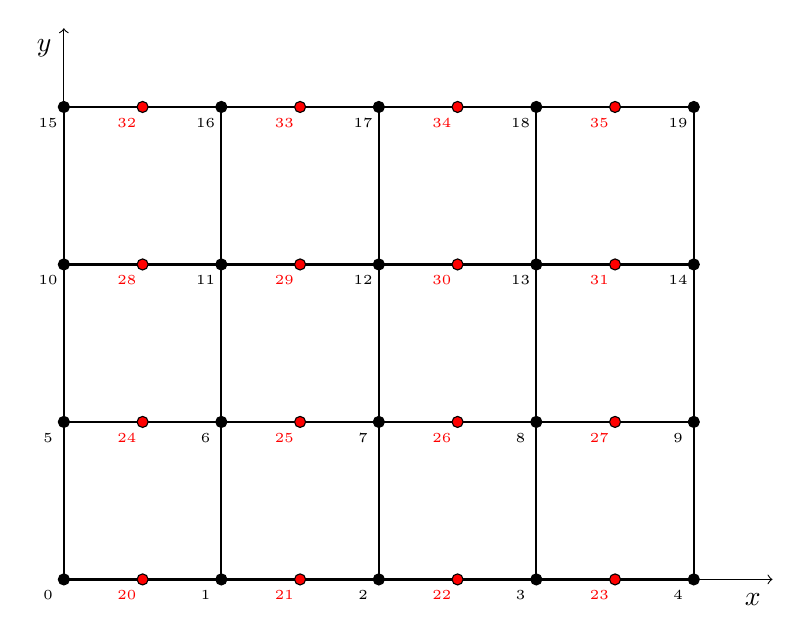
\begin{tikzpicture}
%\draw[fill=gray!23,gray!23](0,0) rectangle (10,8);
%\draw[step=0.5cm,gray,very thin] (0,0) grid (10,8); %background grid

\draw[thick] (1,1) -- (9,1) ;
\draw[thick] (1,3) -- (9,3) ;
\draw[thick] (1,5) -- (9,5) ;
\draw[thick] (1,7) -- (9,7) ;

\draw[thick] (1,1) -- (1,7) ;
\draw[thick] (3,1) -- (3,7) ;
\draw[thick] (5,1) -- (5,7) ;
\draw[thick] (7,1) -- (7,7) ;
\draw[thick] (9,1) -- (9,7) ;

\draw[black,fill=black] (1,1)   circle (2pt);
\draw[black,fill=black] (3,1)   circle (2pt);
\draw[black,fill=black] (5,1)   circle (2pt);
\draw[black,fill=black] (7,1)   circle (2pt);
\draw[black,fill=black] (9,1)   circle (2pt);

\draw[black,fill=black] (1,3)   circle (2pt);
\draw[black,fill=black] (3,3)   circle (2pt);
\draw[black,fill=black] (5,3)   circle (2pt);
\draw[black,fill=black] (7,3)   circle (2pt);
\draw[black,fill=black] (9,3)   circle (2pt);

\draw[black,fill=black] (1,5)   circle (2pt);
\draw[black,fill=black] (3,5)   circle (2pt);
\draw[black,fill=black] (5,5)   circle (2pt);
\draw[black,fill=black] (7,5)   circle (2pt);
\draw[black,fill=black] (9,5)   circle (2pt);

\draw[black,fill=black] (1,7)   circle (2pt);
\draw[black,fill=black] (3,7)   circle (2pt);
\draw[black,fill=black] (5,7)   circle (2pt);
\draw[black,fill=black] (7,7)   circle (2pt);
\draw[black,fill=black] (9,7)   circle (2pt);

\draw[black,fill=red] (2,1) circle (2pt); 
\draw[black,fill=red] (4,1) circle (2pt); 
\draw[black,fill=red] (6,1) circle (2pt); 
\draw[black,fill=red] (8,1) circle (2pt); 

\draw[black,fill=red] (2,3) circle (2pt); 
\draw[black,fill=red] (4,3) circle (2pt); 
\draw[black,fill=red] (6,3) circle (2pt); 
\draw[black,fill=red] (8,3) circle (2pt); 

\draw[black,fill=red] (2,5) circle (2pt); 
\draw[black,fill=red] (4,5) circle (2pt); 
\draw[black,fill=red] (6,5) circle (2pt); 
\draw[black,fill=red] (8,5) circle (2pt); 

\draw[black,fill=red] (2,7) circle (2pt); 
\draw[black,fill=red] (4,7) circle (2pt); 
\draw[black,fill=red] (6,7) circle (2pt); 
\draw[black,fill=red] (8,7) circle (2pt); 

\draw[thin,->] (9,1) -- (10,1); %x
\draw[thin,->] (1,7) -- (1,8); %y
\node[] at (9.75,0.75) {$x$};
\node[] at (0.75,7.75) {$y$};

\node[] at (0.8,0.8) {\tiny 0};
\node[] at (2.8,0.8) {\tiny 1};
\node[] at (4.8,0.8) {\tiny 2};
\node[] at (6.8,0.8) {\tiny 3};
\node[] at (8.8,0.8) {\tiny 4};
\node[] at (0.8,2.8) {\tiny 5};
\node[] at (2.8,2.8) {\tiny 6};
\node[] at (4.8,2.8) {\tiny 7};
\node[] at (6.8,2.8) {\tiny 8};
\node[] at (8.8,2.8) {\tiny 9};
\node[] at (0.8,4.8) {\tiny 10};
\node[] at (2.8,4.8) {\tiny 11};
\node[] at (4.8,4.8) {\tiny 12};
\node[] at (6.8,4.8) {\tiny 13};
\node[] at (8.8,4.8) {\tiny 14};
\node[] at (0.8,6.8) {\tiny 15};
\node[] at (2.8,6.8) {\tiny 16};
\node[] at (4.8,6.8) {\tiny 17};
\node[] at (6.8,6.8) {\tiny 18};
\node[] at (8.8,6.8) {\tiny 19};

\node[] at (1.8,0.8) {\tiny \color{red} 20};
\node[] at (3.8,0.8) {\tiny \color{red} 21};
\node[] at (5.8,0.8) {\tiny \color{red} 22};
\node[] at (7.8,0.8) {\tiny \color{red} 23};

\node[] at (1.8,2.8) {\tiny \color{red} 24};
\node[] at (3.8,2.8) {\tiny \color{red} 25};
\node[] at (5.8,2.8) {\tiny \color{red} 26};
\node[] at (7.8,2.8) {\tiny \color{red} 27};

\node[] at (1.8,4.8) {\tiny \color{red} 28};
\node[] at (3.8,4.8) {\tiny \color{red} 29};
\node[] at (5.8,4.8) {\tiny \color{red} 30};
\node[] at (7.8,4.8) {\tiny \color{red} 31};

\node[] at (1.8,6.8) {\tiny \color{red} 32};
\node[] at (3.8,6.8) {\tiny \color{red} 33};
\node[] at (5.8,6.8) {\tiny \color{red} 34};
\node[] at (7.8,6.8) {\tiny \color{red} 35};

\end{tikzpicture}
\end{center}









\begin{center}
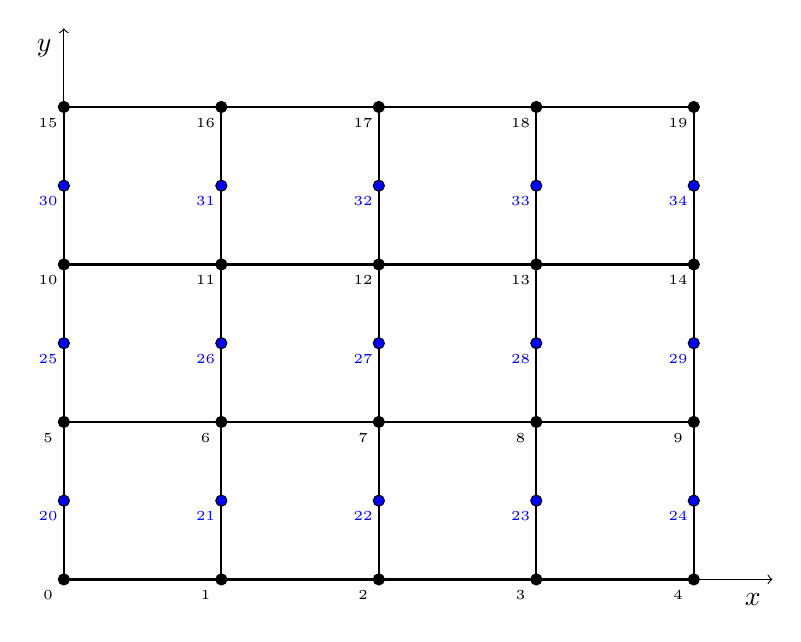
\begin{tikzpicture}
%\draw[fill=gray!23,gray!23](0,0) rectangle (10,8);
%\draw[step=0.5cm,gray,very thin] (0,0) grid (10,8); %background grid

\draw[thick] (1,1) -- (9,1) ;
\draw[thick] (1,3) -- (9,3) ;
\draw[thick] (1,5) -- (9,5) ;
\draw[thick] (1,7) -- (9,7) ;

\draw[thick] (1,1) -- (1,7) ;
\draw[thick] (3,1) -- (3,7) ;
\draw[thick] (5,1) -- (5,7) ;
\draw[thick] (7,1) -- (7,7) ;
\draw[thick] (9,1) -- (9,7) ;

\draw[black,fill=black] (1,1)   circle (2pt);
\draw[black,fill=black] (3,1)   circle (2pt);
\draw[black,fill=black] (5,1)   circle (2pt);
\draw[black,fill=black] (7,1)   circle (2pt);
\draw[black,fill=black] (9,1)   circle (2pt);

\draw[black,fill=black] (1,3)   circle (2pt);
\draw[black,fill=black] (3,3)   circle (2pt);
\draw[black,fill=black] (5,3)   circle (2pt);
\draw[black,fill=black] (7,3)   circle (2pt);
\draw[black,fill=black] (9,3)   circle (2pt);

\draw[black,fill=black] (1,5)   circle (2pt);
\draw[black,fill=black] (3,5)   circle (2pt);
\draw[black,fill=black] (5,5)   circle (2pt);
\draw[black,fill=black] (7,5)   circle (2pt);
\draw[black,fill=black] (9,5)   circle (2pt);

\draw[black,fill=black] (1,7)   circle (2pt);
\draw[black,fill=black] (3,7)   circle (2pt);
\draw[black,fill=black] (5,7)   circle (2pt);
\draw[black,fill=black] (7,7)   circle (2pt);
\draw[black,fill=black] (9,7)   circle (2pt);

\draw[black,fill=blue] (1,2) circle (2pt); 
\draw[black,fill=blue] (3,2) circle (2pt); 
\draw[black,fill=blue] (5,2) circle (2pt); 
\draw[black,fill=blue] (7,2) circle (2pt); 
\draw[black,fill=blue] (9,2) circle (2pt); 

\draw[black,fill=blue] (1,4) circle (2pt); 
\draw[black,fill=blue] (3,4) circle (2pt); 
\draw[black,fill=blue] (5,4) circle (2pt); 
\draw[black,fill=blue] (7,4) circle (2pt); 
\draw[black,fill=blue] (9,4) circle (2pt); 

\draw[black,fill=blue] (1,6) circle (2pt); 
\draw[black,fill=blue] (3,6) circle (2pt); 
\draw[black,fill=blue] (5,6) circle (2pt); 
\draw[black,fill=blue] (7,6) circle (2pt); 
\draw[black,fill=blue] (9,6) circle (2pt); 


\draw[thin,->] (9,1) -- (10,1); %x
\draw[thin,->] (1,7) -- (1,8); %y
\node[] at (9.75,0.75) {$x$};
\node[] at (0.75,7.75) {$y$};

\node[] at (0.8,0.8) {\tiny 0};
\node[] at (2.8,0.8) {\tiny 1};
\node[] at (4.8,0.8) {\tiny 2};
\node[] at (6.8,0.8) {\tiny 3};
\node[] at (8.8,0.8) {\tiny 4};
\node[] at (0.8,2.8) {\tiny 5};
\node[] at (2.8,2.8) {\tiny 6};
\node[] at (4.8,2.8) {\tiny 7};
\node[] at (6.8,2.8) {\tiny 8};
\node[] at (8.8,2.8) {\tiny 9};
\node[] at (0.8,4.8) {\tiny 10};
\node[] at (2.8,4.8) {\tiny 11};
\node[] at (4.8,4.8) {\tiny 12};
\node[] at (6.8,4.8) {\tiny 13};
\node[] at (8.8,4.8) {\tiny 14};
\node[] at (0.8,6.8) {\tiny 15};
\node[] at (2.8,6.8) {\tiny 16};
\node[] at (4.8,6.8) {\tiny 17};
\node[] at (6.8,6.8) {\tiny 18};
\node[] at (8.8,6.8) {\tiny 19};

\node[] at (0.8,1.8) {\tiny \color{blue} 20};
\node[] at (2.8,1.8) {\tiny \color{blue} 21};
\node[] at (4.8,1.8) {\tiny \color{blue} 22};
\node[] at (6.8,1.8) {\tiny \color{blue} 23};
\node[] at (8.8,1.8) {\tiny \color{blue} 24};

\node[] at (0.8,3.8) {\tiny \color{blue} 25};
\node[] at (2.8,3.8) {\tiny \color{blue} 26};
\node[] at (4.8,3.8) {\tiny \color{blue} 27};
\node[] at (6.8,3.8) {\tiny \color{blue} 28};
\node[] at (8.8,3.8) {\tiny \color{blue} 29};

\node[] at (0.8,5.8) {\tiny \color{blue} 30};
\node[] at (2.8,5.8) {\tiny \color{blue} 31};
\node[] at (4.8,5.8) {\tiny \color{blue} 32};
\node[] at (6.8,5.8) {\tiny \color{blue} 33};
\node[] at (8.8,5.8) {\tiny \color{blue} 34};

\end{tikzpicture}
\end{center}








For this mesh we have 

\begin{lstlisting}
nelx=4
nely=3
nnx=nelx+1
nny=nely+1
nel=nelx*nely (=12) 
NP=nel (=12)
Nu=nnx*nny+nnx*nely (=20+16=36)
Nv=nnx*nny+nelx*nny (=20+15=35)
\end{lstlisting}

The total number of velocity dofs is 
\begin{lstlisting}
NfemV=ndofV*nnx*nny + nnx*nely + nny*nelx (=71)
\end{lstlisting}

What makes this element pair rather awkward to implement is the fact that 
there are two connectivity arrays {\tt iconu} and {\tt iconv}, both of size $mV\times nel$, where 
$mV=6$ is the number of nodes linked to an element for each velocity component. 
\begin{itemize}
\item content of {\tt iconu}
\begin{verbatim}
elt
0 | [ 0  1  6  5 20 24]
1 | [ 1  2  7  6 21 25]
2 | [ 2  3  8  7 22 26]
3 | [ 3  4  9  8 23 27]
4 | [ 5  6 11 10 24 28]
5 | [ 6  7 12 11 25 29]
6 | [ 7  8 13 12 26 30]
7 | [ 8  9 14 13 27 31]
8 | [10 11 16 15 28 32]
9 | [11 12 17 16 29 33]
10 | [12 13 18 17 30 34]
11 | [13 14 19 18 31 35]
\end{verbatim}
\item content of {\tt iconv}
\begin{verbatim}
elt
0 | [ 0  1  6  5 20 21]
1 | [ 1  2  7  6 21 22]
2 | [ 2  3  8  7 22 23]
3 | [ 3  4  9  8 23 24]
4 | [ 5  6 11 10 25 26]
5 | [ 6  7 12 11 26 27]
6 | [ 7  8 13 12 27 28]
7 | [ 8  9 14 13 28 29]
8 | [10 11 16 15 30 31]
9 | [11 12 17 16 31 32]
10 | [12 13 18 17 32 33]
11 | [13 14 19 18 33 34]
\end{verbatim}
\end{itemize}

Unlike many other codes in this book the solution vector $\vec{\cal V}$ 
is organised as follows:
\[
\vec{\cal V} = ( u_1, u_2, ... u_{Nu}, v_1, v_2, ... v_{Nv})
\]

As mentioned in the articles\footnote{See also Section~\ref{MMM-ss:qqq_elt}} 
it appears that 
\begin{displayquote}
{\color{darkgray}
It is difficult to find a
local basis for $P_h$. But on the other side, it is the special interest of the method that
the space $P_h$ can be omitted in computation and the discrete solutions approximating
the pressure function in the Stokes equations can be obtained as byproducts, as we
shall see next.}
\end{displayquote}


Remark: given the weird placement of nodes for u and v, it makes sense not to 
use an isoparameteric mapping, and instead choose a Q1 mapping.

Remark: the paper does not mention quadrature at all. 
I choose a 3x3 quadrature as for $Q_2\times Q_1$. 
Should I use a different quadrature for the div-div term?

Remark: the paper also does not mention 3D, nor non-rectangular elements. 

%%%%%%%%%%%%%%%%%%%%%%%%%%%%%%%%%%%%
\section*{Iterated penalty method}

Following \cite{zhan09,huzh11} we implement this method since it 

\begin{displayquote}
{\color{darkgray}
it is the special interest
of the divergence-free finite element method that the space $P_h$ can be omitted
in computation and the discrete solutions approximating the pressure function
in the Stokes equations can be obtained as byproducts, if an iterated penalty
method is adopted to solve system (2.5).}
\end{displayquote}

Also in \cite{huzh11}:
\begin{displayquote}
{\color{darkgray}
We do enough iterated penalty iterations (cf. [25,30]) until the iterative error is smaller
than the truncation error each time.}
\end{displayquote}

In \cite{zhan09} we find:
\begin{center}
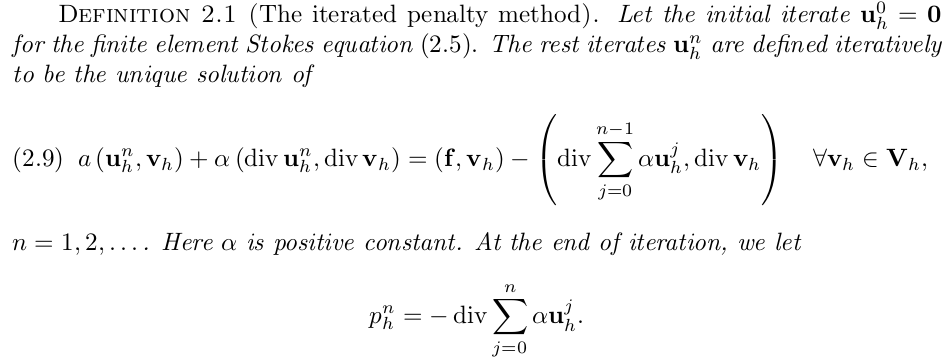
\includegraphics[width=12cm]{python_codes/fieldstone_161/images/iterpen}
\end{center}

Let us then write the first steps of this algorithm\footnote{For personal reasons
and to establish a parallel with the penalty method, I replace $\alpha$ by $\lambda$.}.
\begin{itemize}
\item
For $n=1$:
\begin{eqnarray}
a({\bm u}_h^1,{\bm v}_h) + \lambda (\text{div}\; {\bm u}_h^1, \text{div}\; {\bm v}_h) 
&=& ({\bm f} , {\bm v}_h) - \text{div}\; \left( \lambda {\bm u}_h^0 , \text{div}\; {\bm v}_h \right) \nn\\
p_h^1 &=& - \text{div}\; [\lambda ( {\bm u}_h^0 + {\bm u}_h^1 )]
\end{eqnarray}
\item 
For $n=2$:
\begin{eqnarray}
a({\bm u}_h^2,{\bm v}_h) + \lambda (\text{div}\; {\bm u}_h^2, \text{div}\; {\bm v}_h) 
&=& ({\bm f} , {\bm v}_h) - \text{div}\; \left( \lambda ({\bm u}_h^0 +{\bm u}_h^1 ), \text{div}\; {\bm v}_h \right) \nn\\
p_h^2 &=& - \text{div}\; [\lambda ( {\bm u}_h^0 + {\bm u}_h^1 + {\bm u}_h^2)]
\end{eqnarray}
\end{itemize}

Concretely, we start with ${\bm u}_h^0={\bm 0}$ and we compute the pressure only when the 
iterations have converged, i.e. the inf norm of the difference between two consecutive 
velocity fields is less than a user chosen tolerance:
\begin{lstlisting}
xi_u=np.max(abs(u_prev-u))
xi_v=np.max(abs(v_prev-v))
if xi_u<tol and xi_v<tol:
   break
\end{lstlisting}

Once the velocity field has been obtained the pressure is computed 
at each corner of each element ($Q_{-1}$ representation).
We will see that it is indeed discontinuous.


\newpage
%==========================================
\section*{grids and dofs}

In \cite{huzh11} we find the following table:

\begin{center}
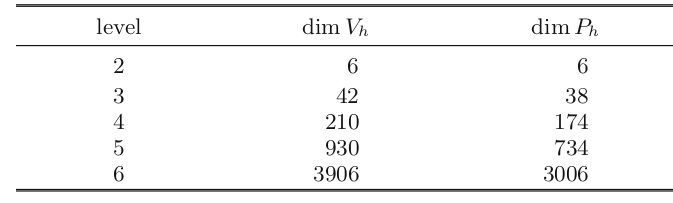
\includegraphics[width=8cm]{python_codes/fieldstone_161/images/dofs}
\end{center}

The authors state that ``The initial grid, level one grid, is simply one unit square''
so that the level 2 grid is a 2x2 element grid:
\begin{verbatim}
+-----+-----+
|     |     |
|     |     |
|     |     |
+-----+-----+
|     |     |
|     |     |
|     |     |
+-----+-----+
\end{verbatim}
with the following velocity dofs:
\begin{verbatim}
U--U--U--U--U   V-----V-----V
|     |     |   |     |     |
|     |     |   V     V     V
|     |     |   |     |     |
U--U--U--U--U   V-----V-----V
|     |     |   |     |     |
|     |     |   V     V     V
|     |     |   |     |     |
U--U--U--U--U   V-----V-----V
\end{verbatim}
Since $u=v=0$ on all boundaries we replace the U,V dofs by x
to indicate that these are no longer degrees of freedom:
\begin{verbatim}
x--x--x--x--x   x-----x-----x
|     |     |   |     |     |
|     |     |   x     V     x
|     |     |   |     |     |
x--U--U--U--x   x-----V-----x
|     |     |   |     |     |
|     |     |   x     V     x
|     |     |   |     |     |
x--x--x--x--x   x-----x-----x
\end{verbatim}
and we indeed find $\text{dim}~V_h=6$. 

Turning now to pressure dofs, it is supposed to be discontinuous Q1, 
so I would expect 4x4=16 dofs. 
Yet, the authors report 6(!) dofs... 

In \cite{huzh11} we read: ``Meanwhile, we decrease the space $Q_1^{dc}$ 
for the pressure to $Q_1'$, by removing all spurious modes, i.e.,
eliminating one degree of freedom at each vertex.
We have to emphasize
that the discrete pressure space is introduced for the analysis, but not in the
computation. By an iterated penalty method, we obtain the discrete solutions
for the pressure without coding the pressure element
''

I do not understand this at all. Even removing 1 pdof per element, there are 3 left
per element, i.e. 12 in total.



%==========================================
\section*{Manufactured solutions}

In \textcite{huzh11} (2011) the authors propose the 
following manufactured solution\footnote{I have removed th $2^8 term$}:

\[
g(x,y)=(x-x^2)^2(y-y^2)^2 =  f(x)h(y)
\]
The velocity is given by 
\[
\vec\upnu 
= 
\left(
\begin{array}{c}
g_y \\ -g_x
\end{array}
\right)
=
\left(
\begin{array}{c}
fh' \\
-f'h
\end{array}
\right)
%=
%\left(
%\begin{array}{c}
%2^9(x-x^2)^2(1-2y)(y-y^2) \\
%-2^9(1-2x)(x-x^2)(y-y^2)^2 
%\end{array}
%\right)
\]
and the pressure is defined as
\[
p
= -g_{xx}
= -f'' h
\]
We have (assuming viscosity is 1) 
\[
\vec{f} = -\Delta \vec{\upnu} + \vec\nabla p
%= 
%\left(
%\begin{array}{c}
%- \Delta g_{y} -g_{xxx}\\
%- \Delta g_{x} -g_{yxx}
%\end{array}
%\right)
%= 
%\left(
%\begin{array}{c}
%- g_{yxx} - g_{yyy} -g_{xxx}\\
%  g_{xxx} + g_{xyy} -g_{yxx}
%\end{array}
%\right)
=
\left(
\begin{array}{c}
- \Delta (fh') -f''' h  \\
-\Delta (-f'h) -f''h'
\end{array}
\right)
=
\left(
\begin{array}{c}
- f''h' - fh''' -f''' h  \\
 f'''h + f'h''  -f''h'
\end{array}
\right)
\]
with
\begin{eqnarray}
f(x)&=& (x-x^2)^2 \nn\\
f'(x) &=& 2(1-2x)(x-x^2) \nn\\
f''(x) &=& 2(1-6x+6x^2) \nn\\
f'''(x) &=& 24x-12 \nn
\end{eqnarray}


\begin{center}
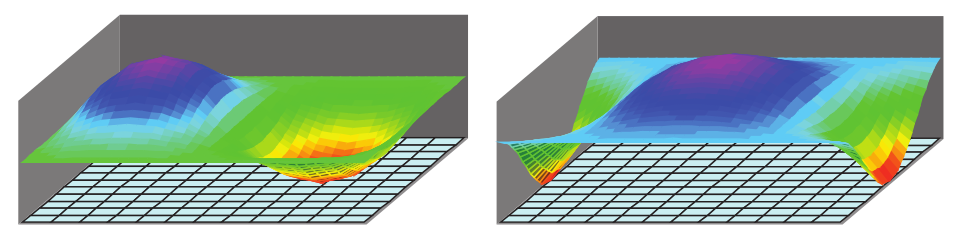
\includegraphics[width=12cm]{python_codes/fieldstone_161/images/mms}\\
{\captionfont Taken from \cite{zhan09}. Second component of velocity and pressure fields.}
\end{center}

\begin{center}
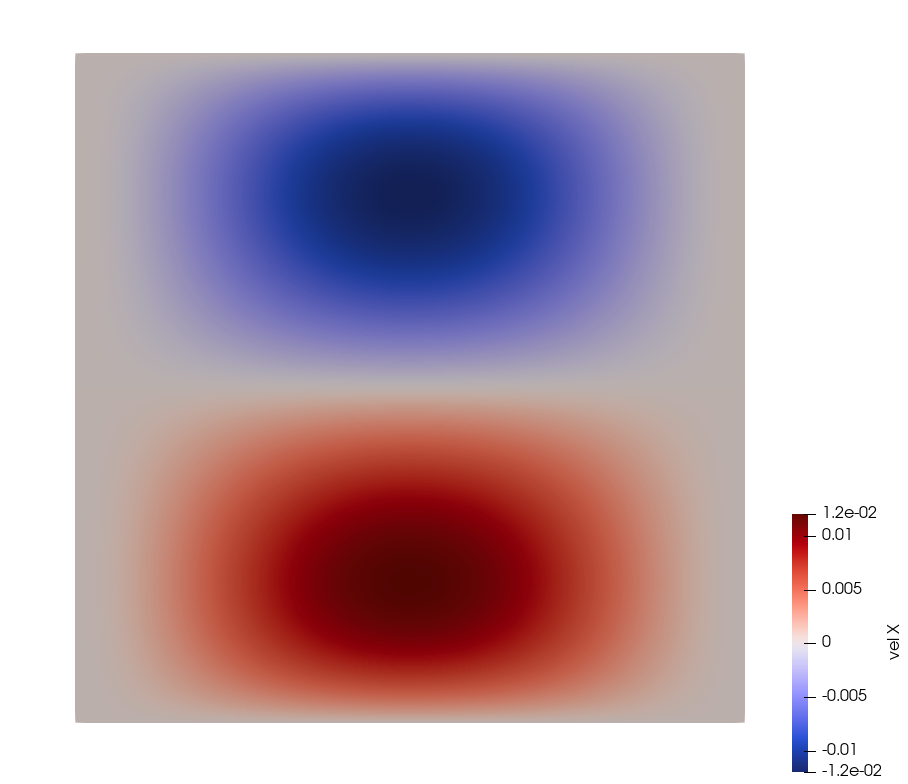
\includegraphics[width=5cm]{python_codes/fieldstone_161/results/bench2/th_u}
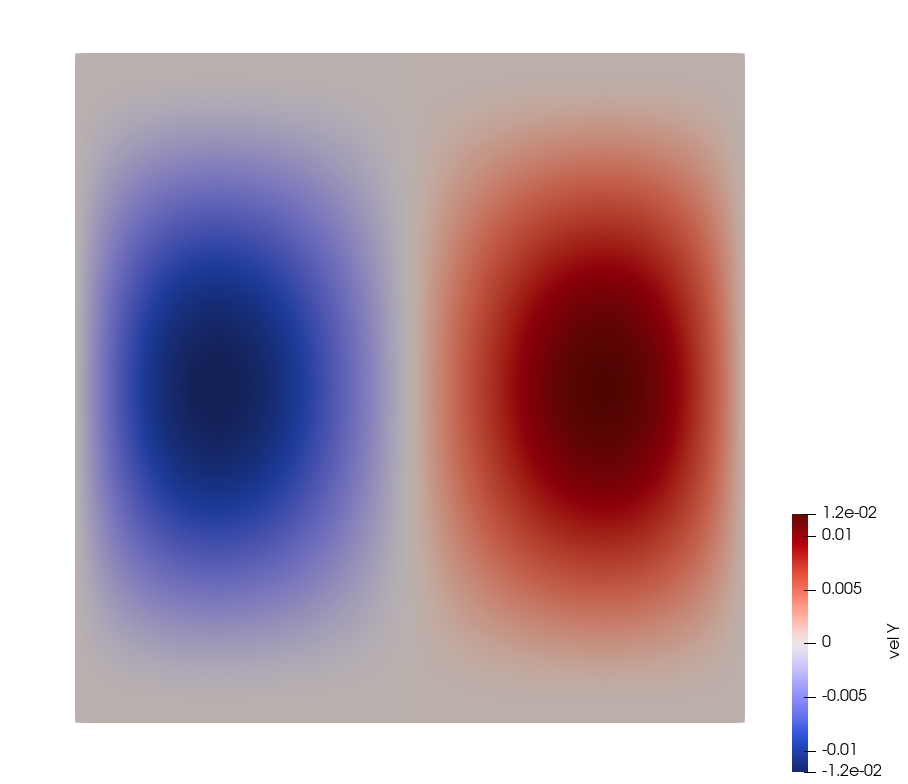
\includegraphics[width=5cm]{python_codes/fieldstone_161/results/bench2/th_v}\\
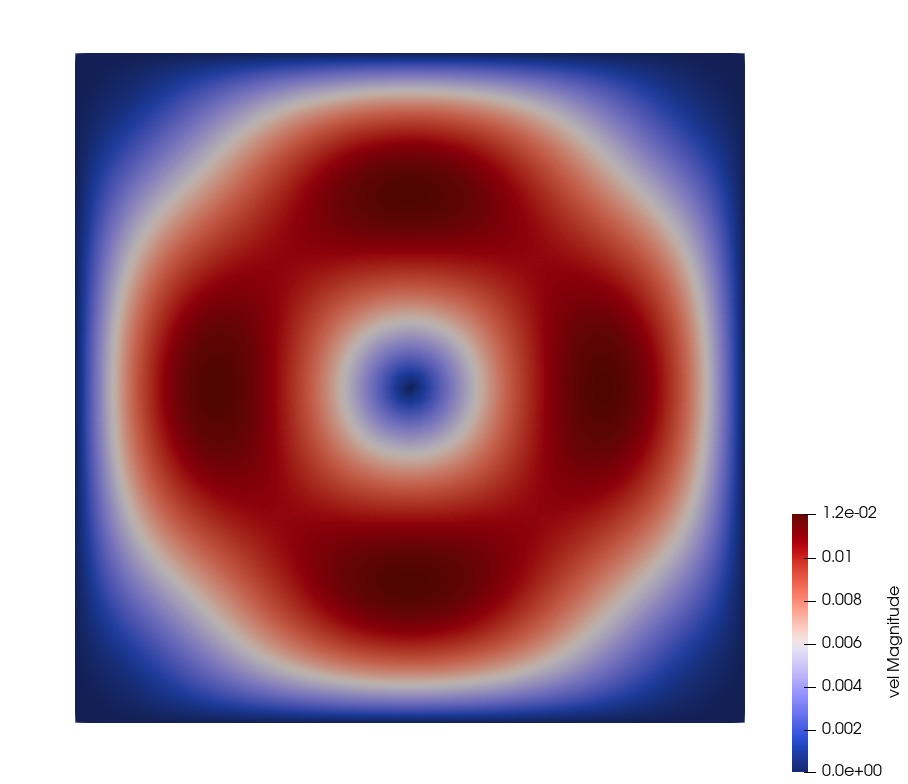
\includegraphics[width=5cm]{python_codes/fieldstone_161/results/bench2/th_vel}
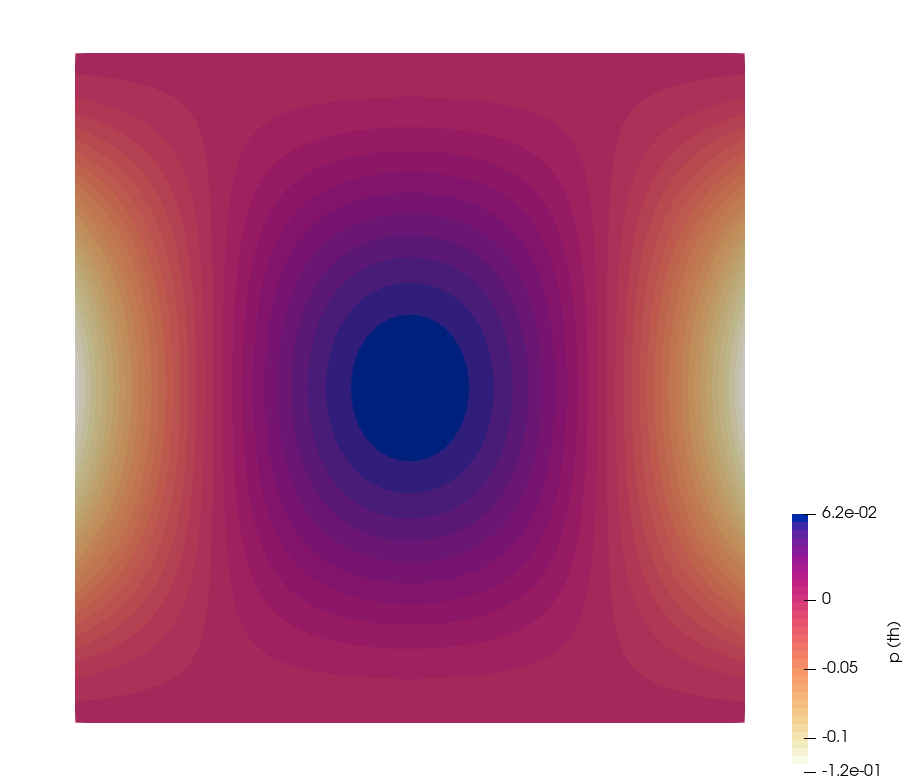
\includegraphics[width=5cm]{python_codes/fieldstone_161/results/bench2/th_press}
\end{center}


They also report the following rates:

\begin{center}
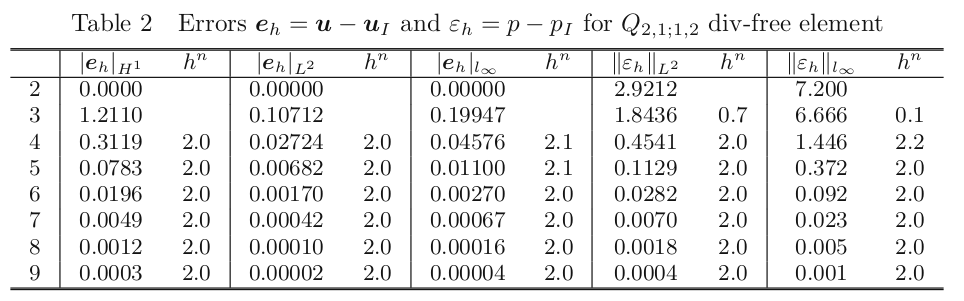
\includegraphics[width=12cm]{python_codes/fieldstone_161/images/errors}
\end{center}

It is quite remarkable that the error convergence rates (in the $L_2$ norm)
are identical for both velocity and pressure. 







\newpage
%============================
\section*{Results}

%------------------------------------------------------------
\subsection*{Donea \& Huerta manufactured solution (bench=1)}

\subsubsection*{Without iterations}

Let us first explore the influence of the $\lambda$ parameter:

\begin{center}
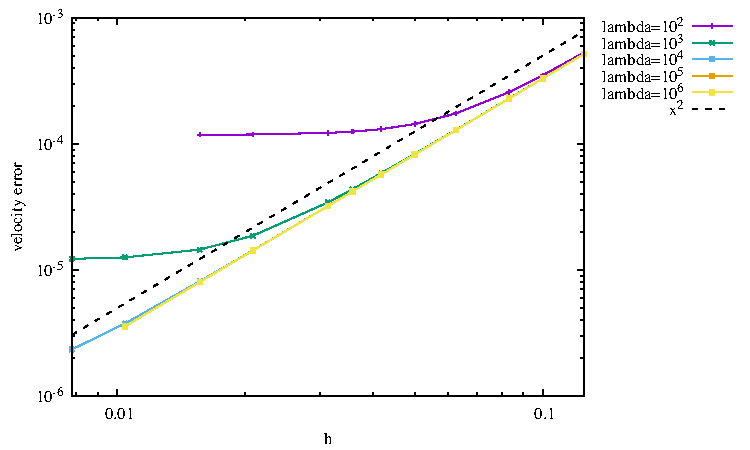
\includegraphics[width=8cm]{python_codes/fieldstone_161/results/bench1/single/errorsV.pdf}
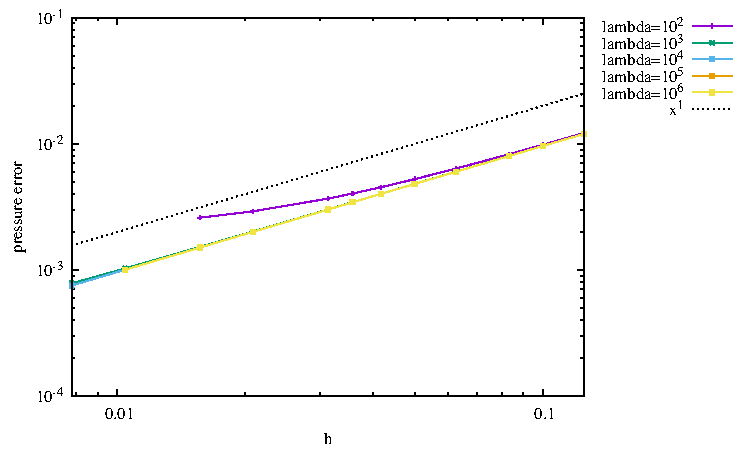
\includegraphics[width=8cm]{python_codes/fieldstone_161/results/bench1/single/errorsP.pdf}\\
\end{center}

\subsubsection*{With iterations}

\begin{center}
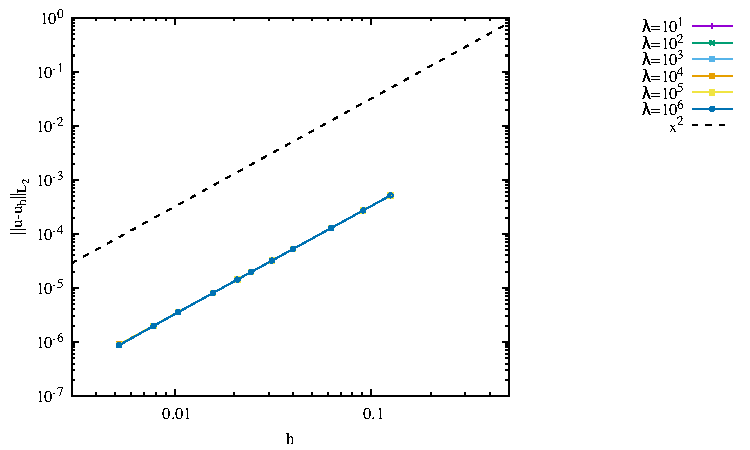
\includegraphics[width=8cm]{python_codes/fieldstone_161/results/bench1/iterations/errorsV.pdf}
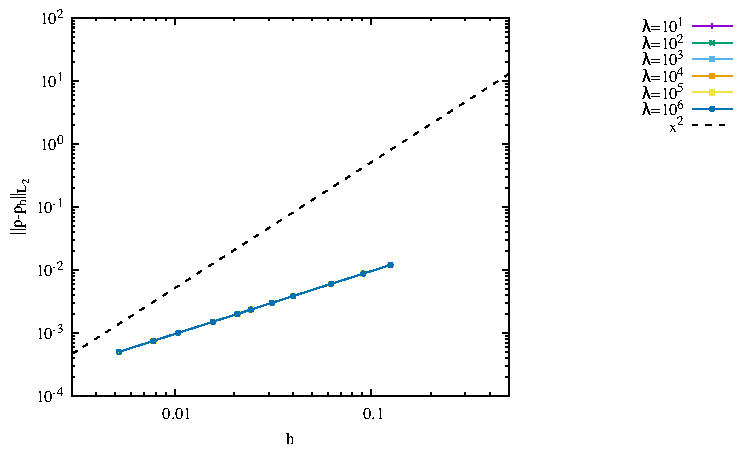
\includegraphics[width=8cm]{python_codes/fieldstone_161/results/bench1/iterations/errorsP.pdf}\\
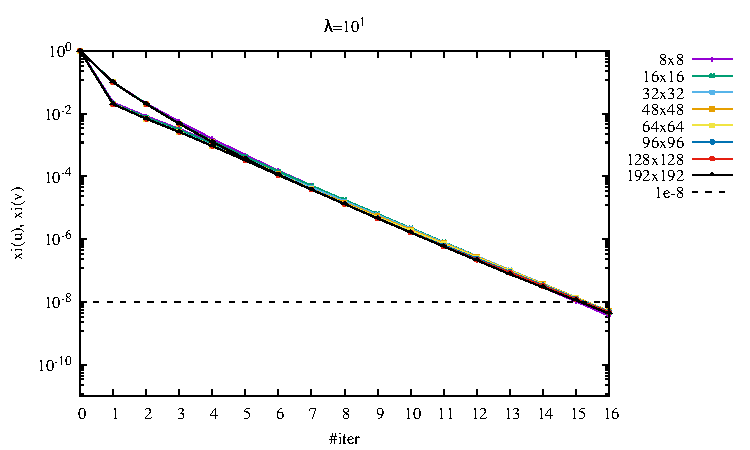
\includegraphics[width=5.7cm]{python_codes/fieldstone_161/results/bench1/iterations/conv1.pdf}
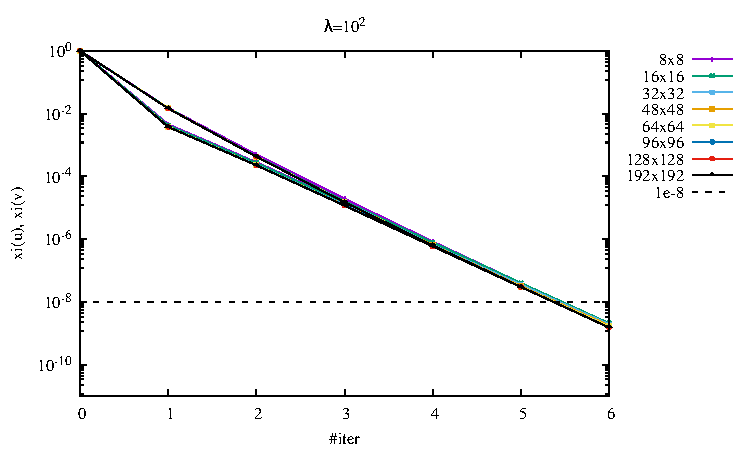
\includegraphics[width=5.7cm]{python_codes/fieldstone_161/results/bench1/iterations/conv2.pdf}
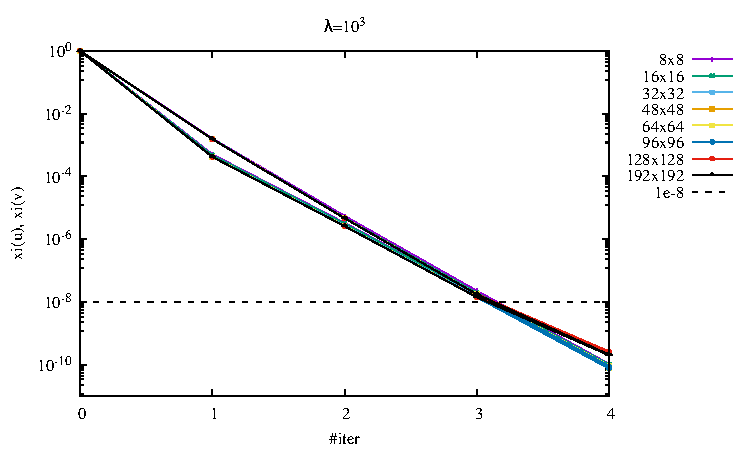
\includegraphics[width=5.7cm]{python_codes/fieldstone_161/results/bench1/iterations/conv3.pdf}\\
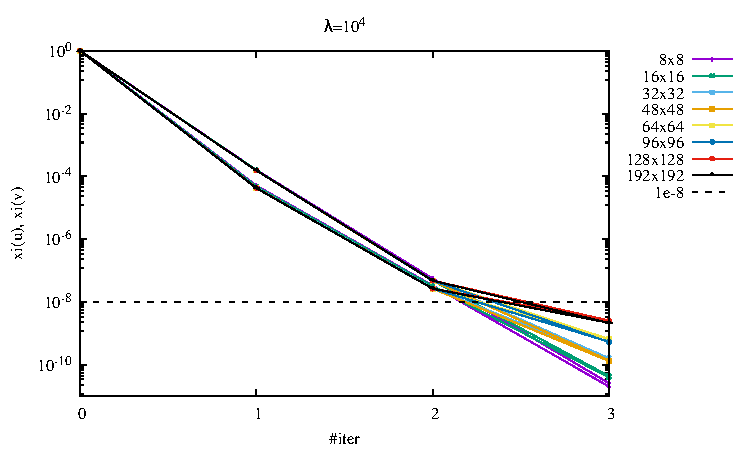
\includegraphics[width=5.7cm]{python_codes/fieldstone_161/results/bench1/iterations/conv4.pdf}
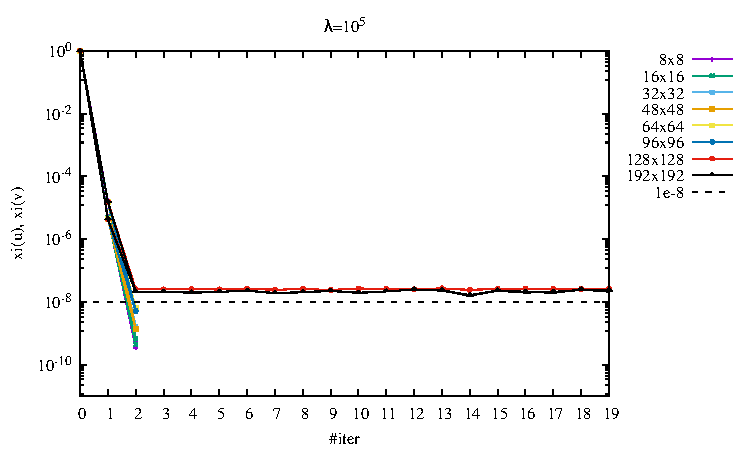
\includegraphics[width=5.7cm]{python_codes/fieldstone_161/results/bench1/iterations/conv5.pdf}
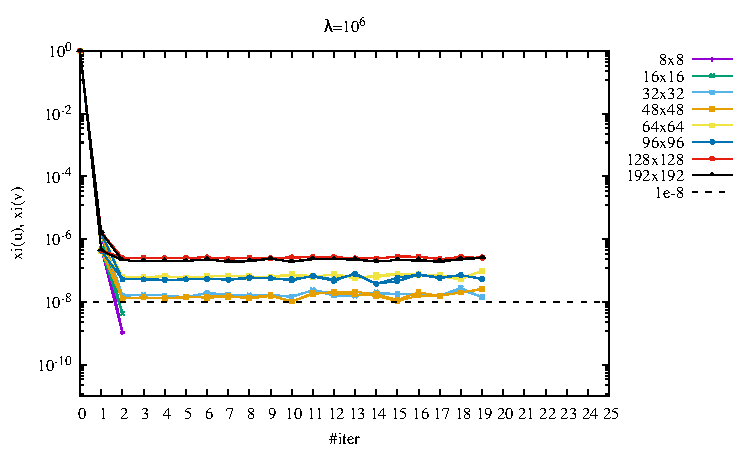
\includegraphics[width=5.7cm]{python_codes/fieldstone_161/results/bench1/iterations/conv6.pdf}
\end{center}

Q: rates are not what is expected from Q2Q1. 
Also huzh11 report 2 and 2 rates in L2 norm.

We find that for $\lambda \ge 10^2$ the number of iterations becomes really small.
Also the number of iterations to reach convergence decreases when $\lambda$ increases. 
Any value higher than $10^4$ does not improve the convergence.

%------------------------------------------------------------ 
\subsection*{Huang \& Zhang manufactured solution (bench=2)}

\begin{center}
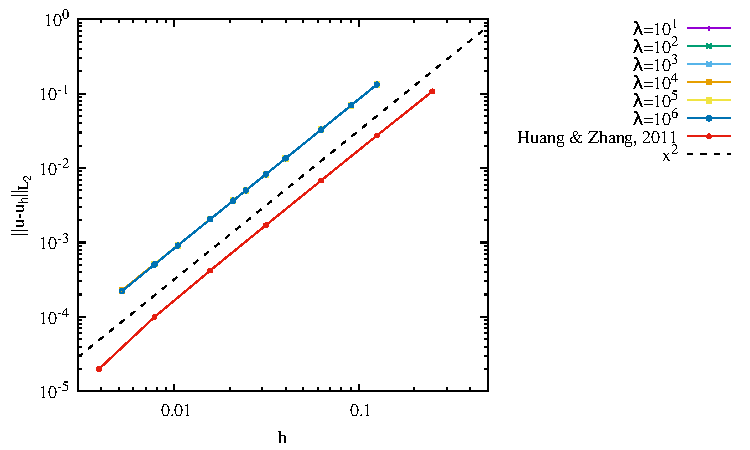
\includegraphics[width=8cm]{python_codes/fieldstone_161/results/bench2/errorsV.pdf}
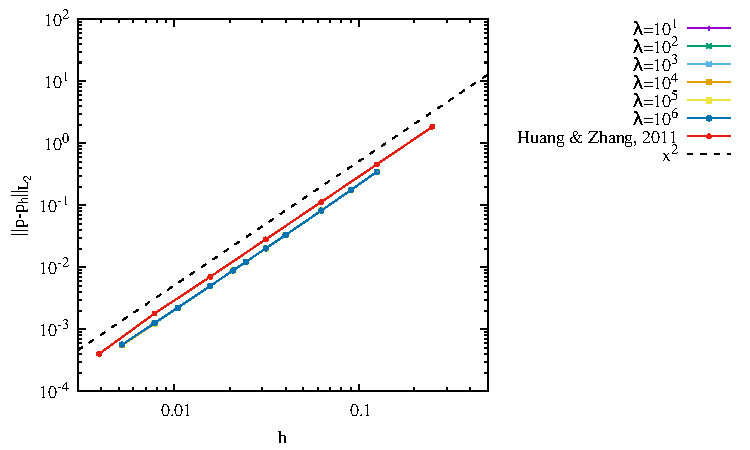
\includegraphics[width=8cm]{python_codes/fieldstone_161/results/bench2/errorsP.pdf}\\
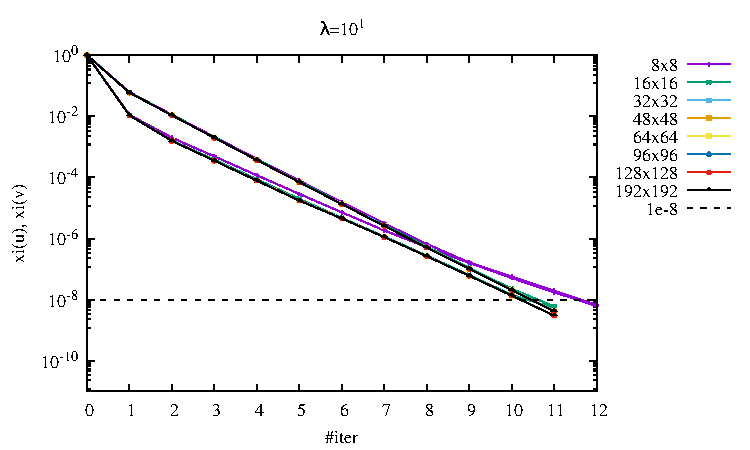
\includegraphics[width=5.7cm]{python_codes/fieldstone_161/results/bench2/conv1.pdf}
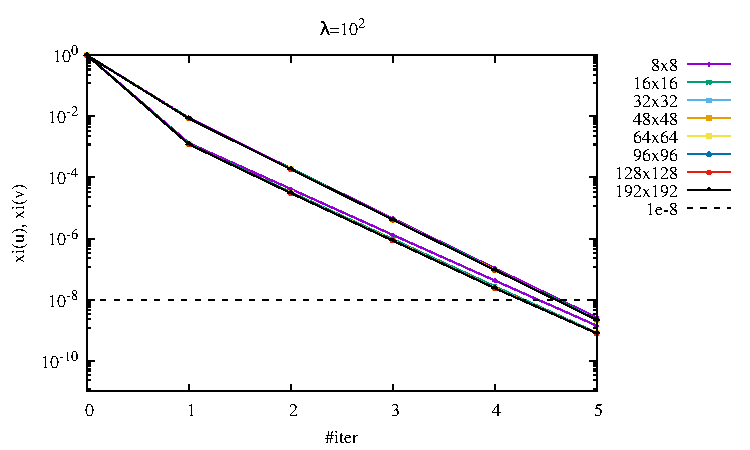
\includegraphics[width=5.7cm]{python_codes/fieldstone_161/results/bench2/conv2.pdf}
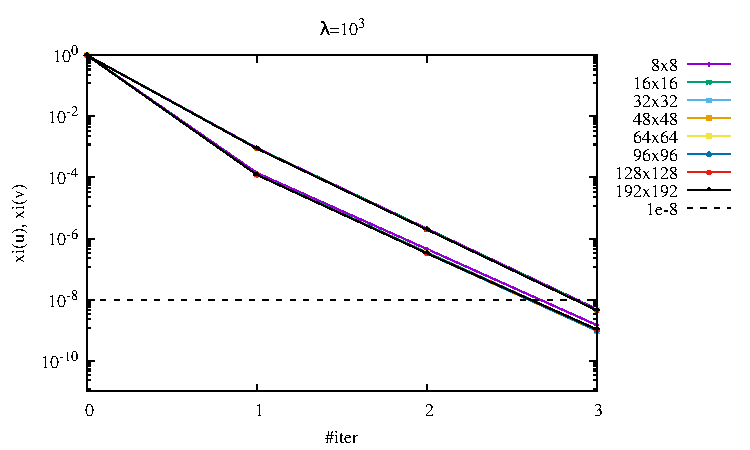
\includegraphics[width=5.7cm]{python_codes/fieldstone_161/results/bench2/conv3.pdf}\\
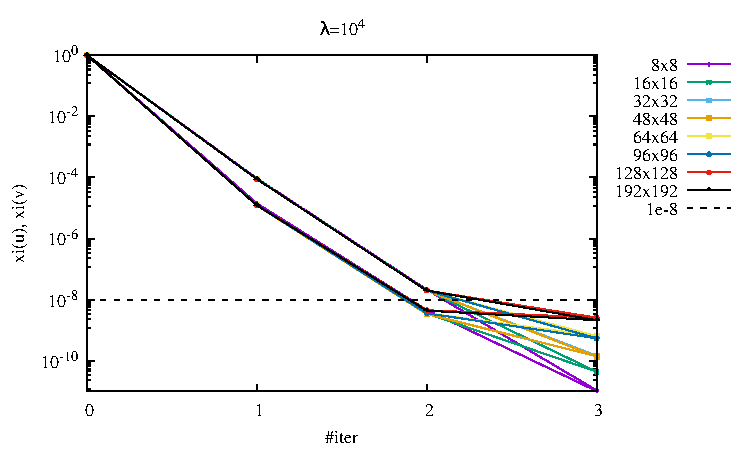
\includegraphics[width=5.7cm]{python_codes/fieldstone_161/results/bench2/conv4.pdf}
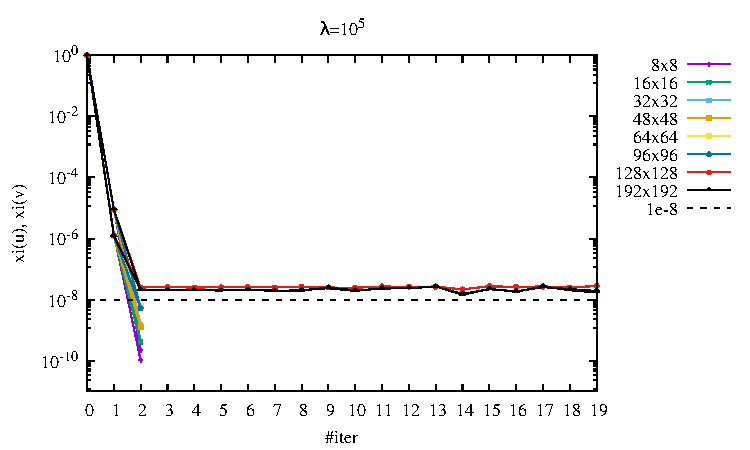
\includegraphics[width=5.7cm]{python_codes/fieldstone_161/results/bench2/conv5.pdf}
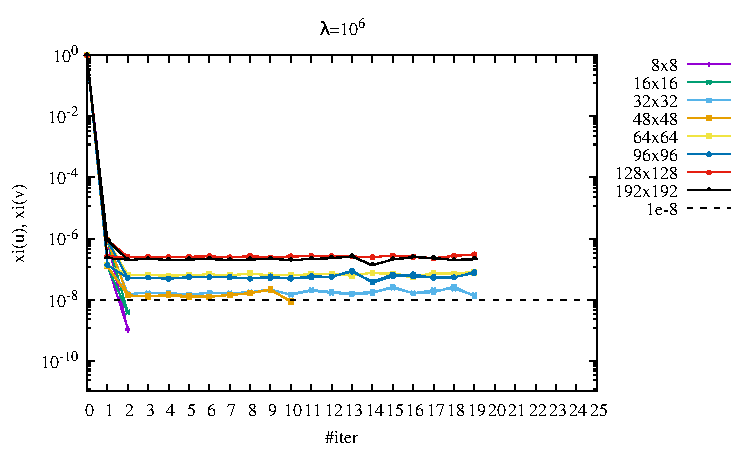
\includegraphics[width=5.7cm]{python_codes/fieldstone_161/results/bench2/conv6.pdf}
\end{center}

This time, we do recover second order convergence rate for pressure?!
Note that at high resolution the case $\lambda=10^6$ fails to converge to the 
desired tolerance. 


\begin{center}
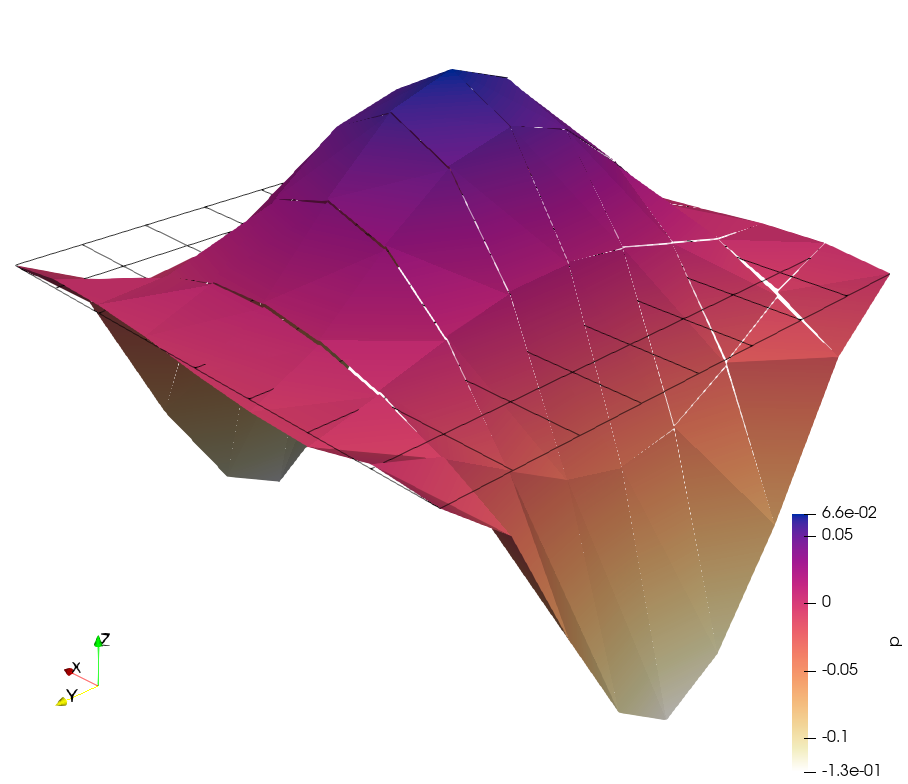
\includegraphics[width=5cm]{python_codes/fieldstone_161/results/bench2/press}
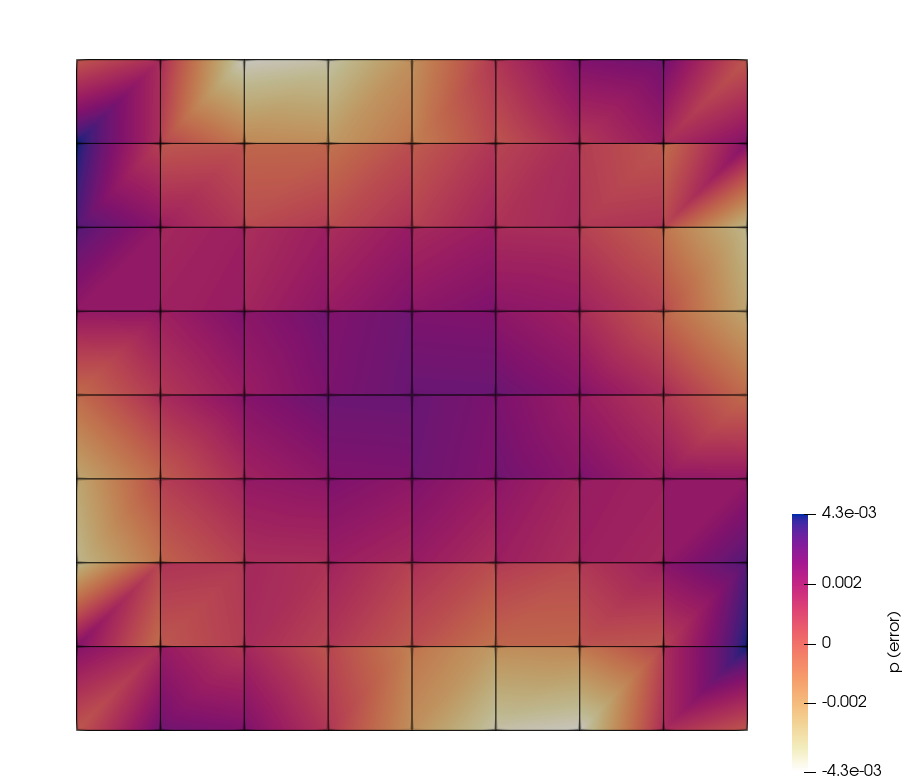
\includegraphics[width=5cm]{python_codes/fieldstone_161/results/bench2/press_error}
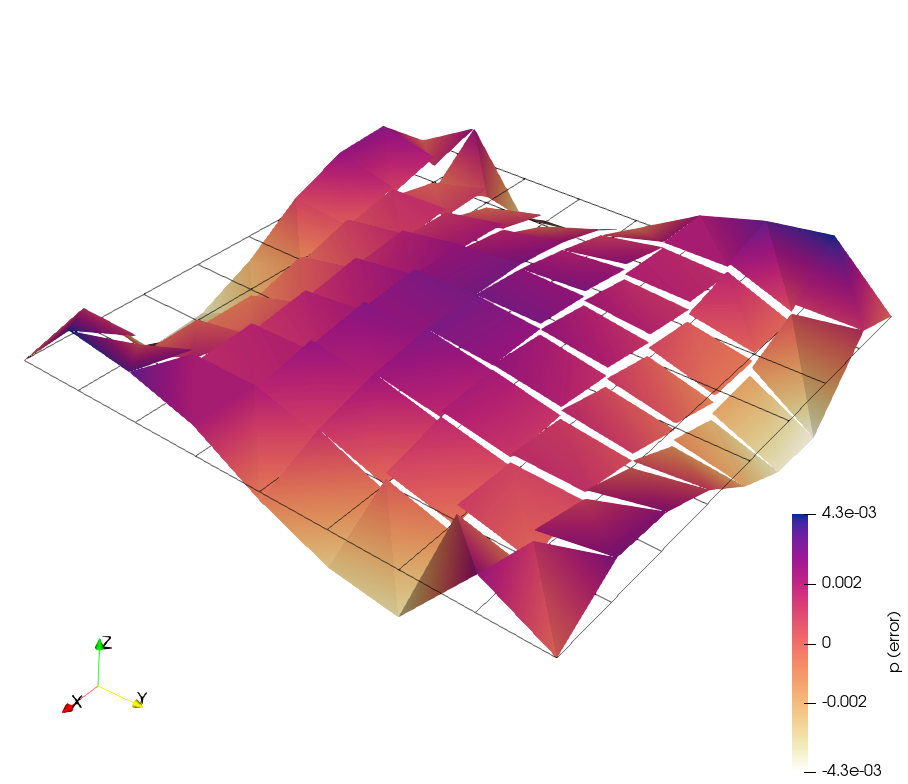
\includegraphics[width=5cm]{python_codes/fieldstone_161/results/bench2/press_error2}\\
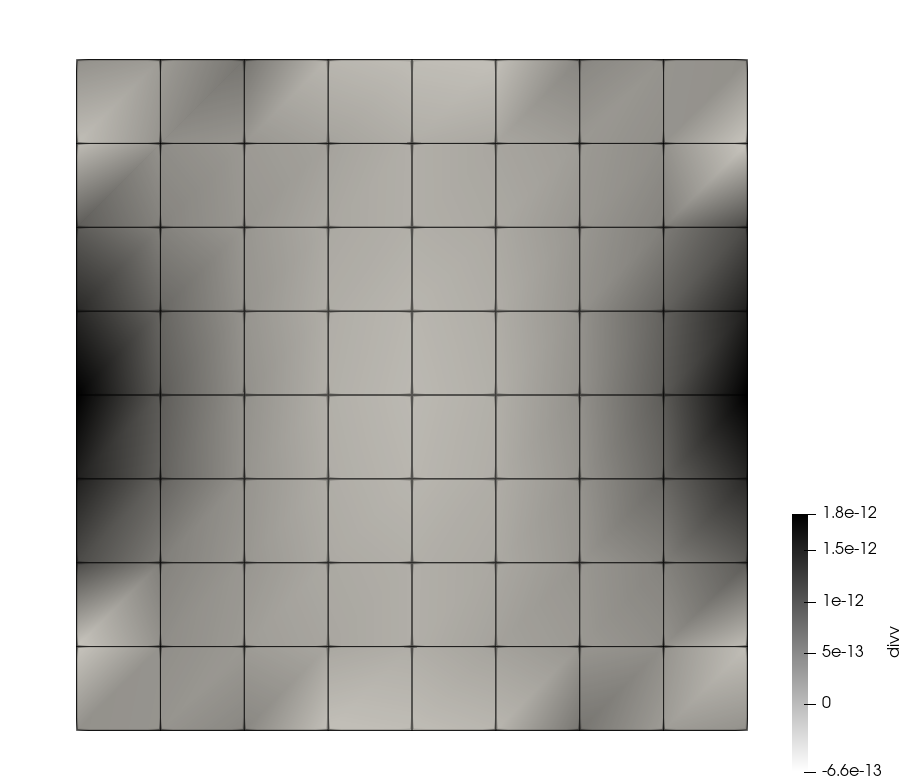
\includegraphics[width=5cm]{python_codes/fieldstone_161/results/bench2/divv}
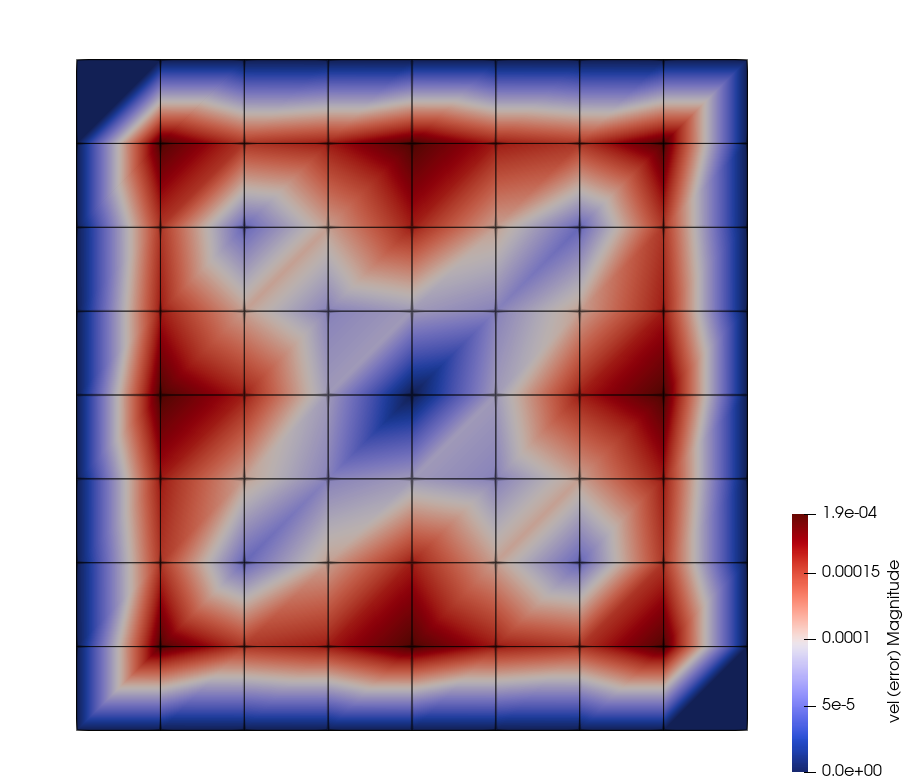
\includegraphics[width=5cm]{python_codes/fieldstone_161/results/bench2/vel_error}\\
{\captionfont Obtained on 8x8 grid. We find that the divergence is indeed very low.
Note that Paraview is misleading: it looks like the squares are divived into 2 triangles but
in reality it is a visualisation artefact!}
\end{center}
It looks like pressure is continuous on the edges of the domain!

